\section*{Simulating the model using Comsol}
\hspace{\parindent} Simulating the model using the Corona discharge previously defined package in Comsol was somehow a challenging task, but we could get some results as we did the following:
\begin{enumerate}
    \item Studying the plasma module (the module specified to simulate corona discharge)
    \item Defining the constants and parameters usually used in the simulation
    \item Setting all the required chemical reactions, including:
            \begin{enumerate}
                \item Electron impact reactions
                \item Surface reactions
                
            \end{enumerate}
    \item Setting the initial values 
    \item Setting the boundary conditions 
    \item Adjusting the meshing to solve by finite volume method (which is preferable for the software)
    \item Adjusting time dependency to take results in different instants
    
\end{enumerate}
\hspace{\parindent}After all of this, we could get results, but what was disappointing is that we couldn't get results except for the 1D model, as the other 2D and 3D models have failed due to both technical and informatics problems.
\hspace{\parindent}From these results, we could calculate the current density at the applied voltage we did in the hardware and got to compare them in the analysis section.

\subsubsection*{Results of the simulation}
\begin{figure}[p]
	\centering
	\includegraphics[scale=0.3]{images/results images/Comsol images/log of positive ion density.png}
	\caption{log of positive ion density}
\end{figure}
\begin{figure}[p]
	\centering
	\includegraphics[scale=0.4]{images/results images/Comsol images/log of negative ion density.png}
	\caption{log of negative ion density
	support}
\end{figure}
\begin{figure}[p]
	\centering
	\includegraphics[scale=0.4]{images/results images/Comsol images/log of electron density.png}
	\caption{log of electron density
	support}
\end{figure}

\begin{figure}[p]
	\centering
	\includegraphics[scale=0.25]{images/results images/Comsol images/Electric potential.png}
	\caption{Electric potential vs r coordinate
	support}
\end{figure}

\begin{figure}[p]
	\centering
	\includegraphics[scale=0.25]{images/results images/Comsol images/Electron density.png}
	\caption{Electron density vs r coordinate
	support}
\end{figure}


\begin{figure}[p]
	\centering
	\includegraphics[scale=0.25]{images/results images/Comsol images/reduced electric field.png}
	\caption{Reduced electric field vs r coordinate
	support}
\end{figure}
\begin{figure}[p]
	\centering
	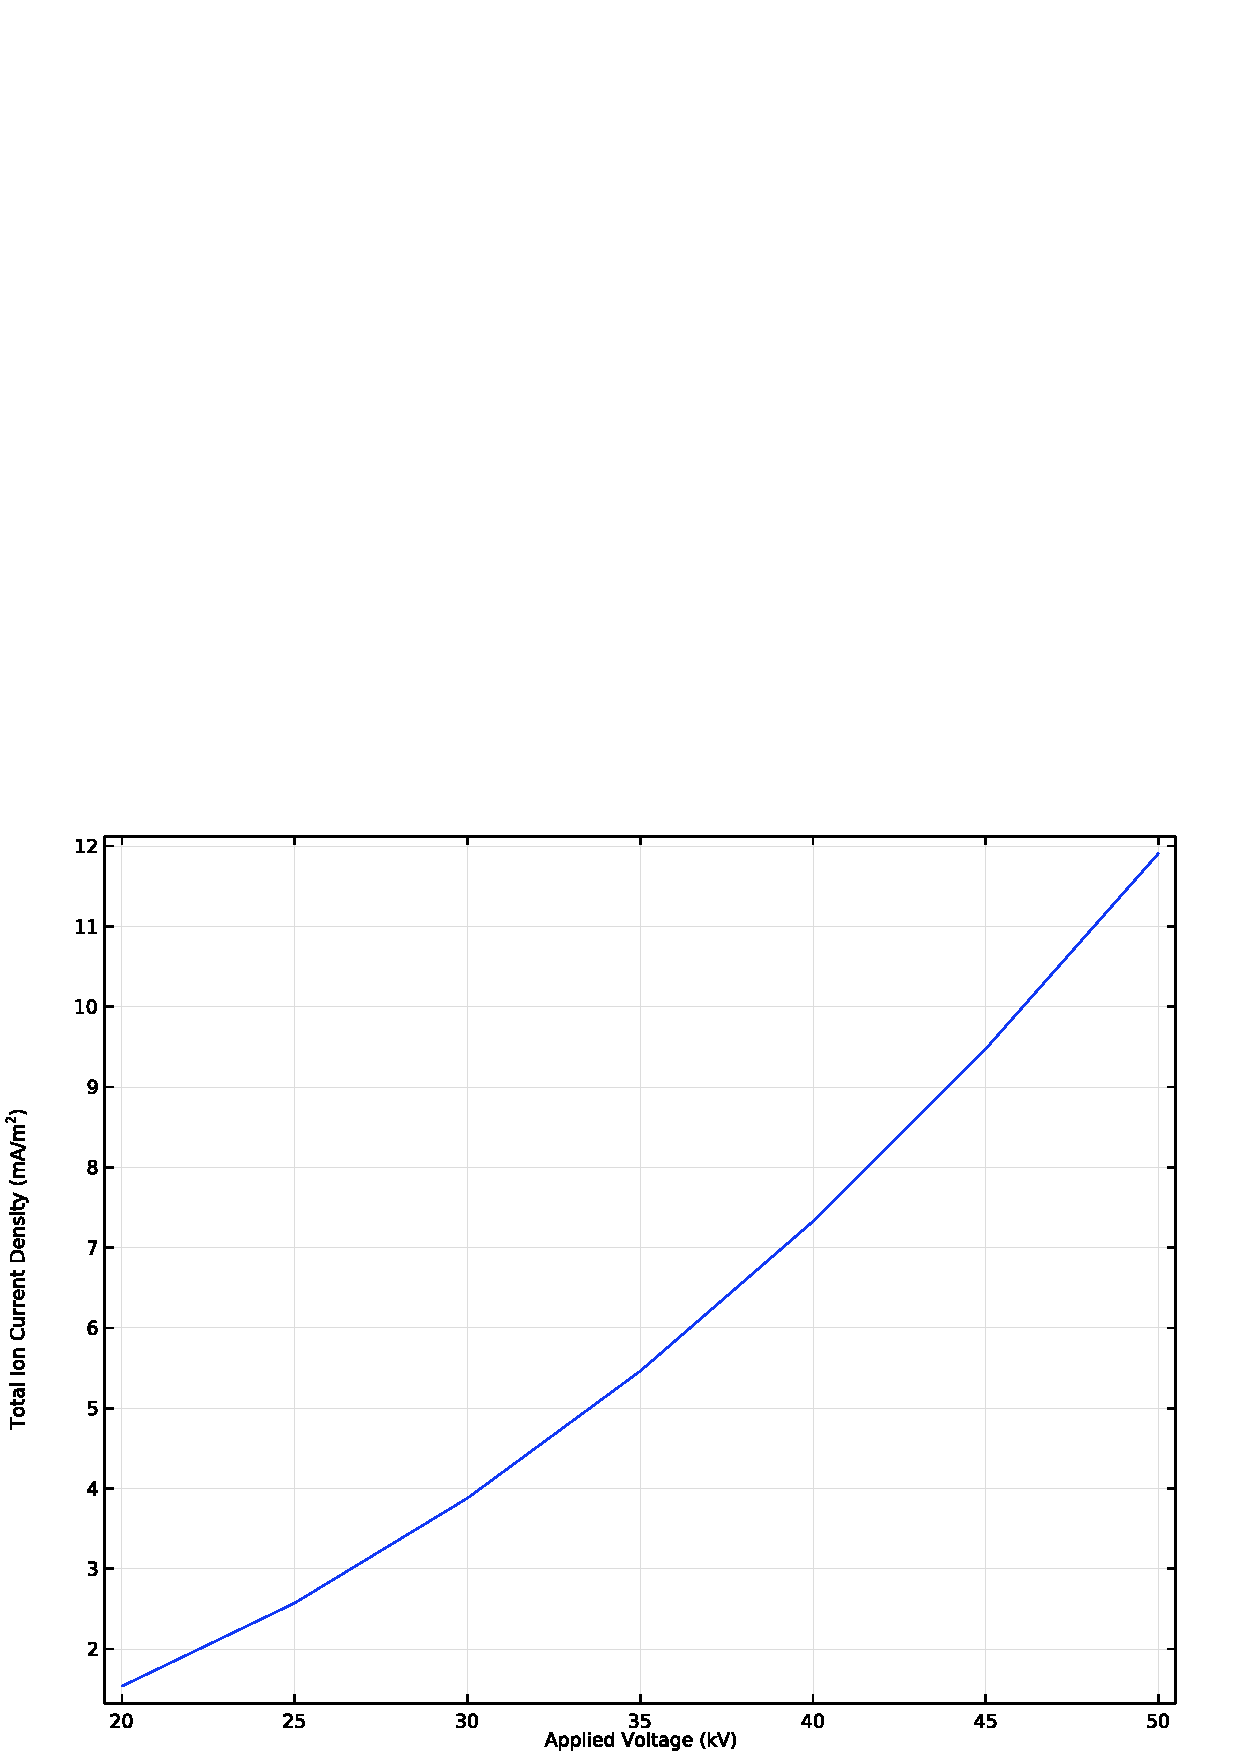
\includegraphics[scale=0.25]{images/results images/Comsol images/total ion current density.png}
	\caption{Total ion current density vs applied voltage
	support}
\end{figure}
